\chapter{Introduction}

%
% ***************************************************************************
%             Formatting: Equations, Tables, Figures, Algorithms
% ***************************************************************************
%
% This section of the template contains some basic formatting instructions
% for formatting algorithms, equations, figures, and tables.
%
% In following chapters you will find some more examples.
%
%****************************************************************************
%

\noindent   % First paragraph has no indentation.
First paragraph in current heading. First paragraph in current heading.
First paragraph in current heading. First paragraph in current heading.
First paragraph in current heading. First paragraph in current heading.
First paragraph in current heading. First paragraph in current heading.
First paragraph in current heading.\cite{article-one}

%
% ********************************************
%         Formatting: Equations
% ********************************************
%
% A sample equation in equation environment:
%

Next paragraph in current heading. Next paragraph in current heading.
Next paragraph in current heading. Next paragraph in current heading.
Next paragraph in current heading. Next paragraph in current heading.
Next paragraph in current heading. Next paragraph in current heading.
Next paragraph in current heading.\cite{article-many,book-knownauthor,book-unknownauthor}

%%
\begin{equation}
\mathrm{\sigma ' = \varepsilon '' \varepsilon _{0} \omega}
\label{eq:sample}
\end{equation}
%%

Next paragraph in current heading. Next paragraph in current heading.
Next paragraph in current heading. Next paragraph in current heading.
Next paragraph in current heading. Next paragraph in current heading.
Next paragraph in current heading. Next paragraph in current heading.
Next paragraph in current heading.

%
% If fractions inside fractions are used, their font gets smaller until they have reached the \scriptstyle limit.
% In order to keep the size consistent, you can declare each fraction to use the display style instead, e.g. by using
% the \displaystyle command:
%

%%
\begin{equation}
x = a_0 + \frac{1}{\displaystyle a_1
+ \frac{1}{\displaystyle a_2
+ \frac{1}{\displaystyle a_3 + a_4}}}
\label{eq:fractions}
\end{equation}
%%

%
% For samples on arrays, matrices, breaking equations into several lines, etc., see
% http://en.wikibooks.org/wiki/LaTeX/Mathematics
%
% ********************************************
% ********************************************
%

Next paragraph in current heading. Next paragraph in current heading.
Next paragraph in current heading. Next paragraph in current heading.
Next paragraph in current heading. Next paragraph in current heading.
Next paragraph in current heading. Next paragraph in current heading.
Next paragraph in current heading.

% ********************************************
%         Formatting: Figures
% ********************************************
%
% Figures in figurename.eps format are supported in LaTeX.
% File subdirectory images contains figures used in the template.
%

%%
\begin{figure}[h!]
\centering
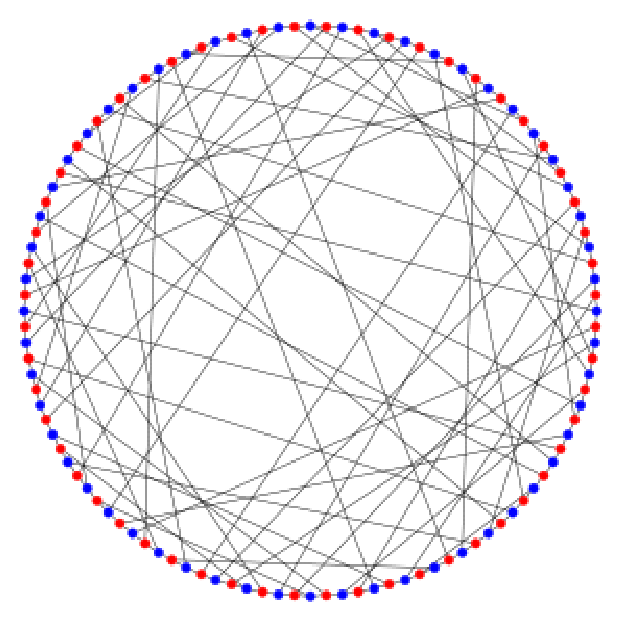
\includegraphics[width=6cm]{sample-1.eps}
\caption[Title]{\textit{Title.} Caption of this figure. Caption of this figure. Caption of this figure.
Caption of this figure. Caption of this figure. Caption of this figure. Caption of this figure. Caption of this figure.}
\label{fig:smiley}
\end{figure}
%%

%
% Using book documentclass, LaTeX automatically centers captions that fit into single line.
% This can be over-ruled by using justification:
% singlelinecheck=<bool>
% it switches the extra centering off by inserting false, no, off or 0 for <bool>
%

Next paragraph in current heading. Next paragraph in current heading.
Next paragraph in current heading. Next paragraph in current heading.
Next paragraph in current heading. Next paragraph in current heading.
Next paragraph in current heading. Next paragraph in current heading.
Next paragraph in current heading.

%

%%
\begin{figure}[h!]
\centering
\subfigure[]{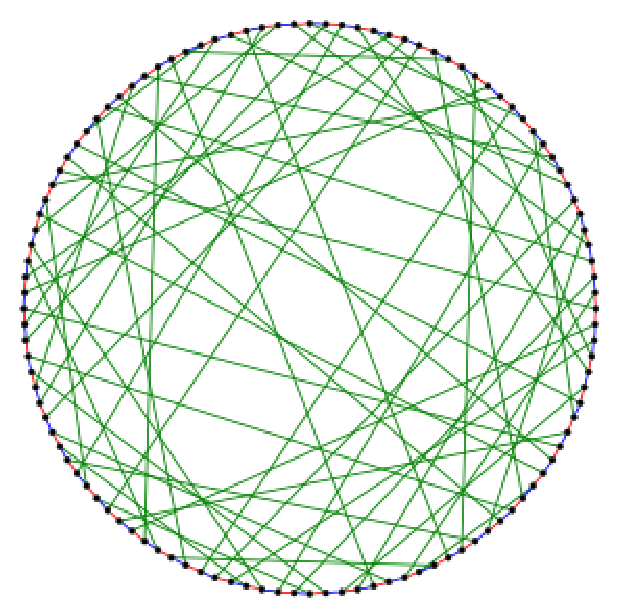
\includegraphics[width=5.5cm]{sample-2a.eps}}
\hspace{10mm}
\subfigure[]{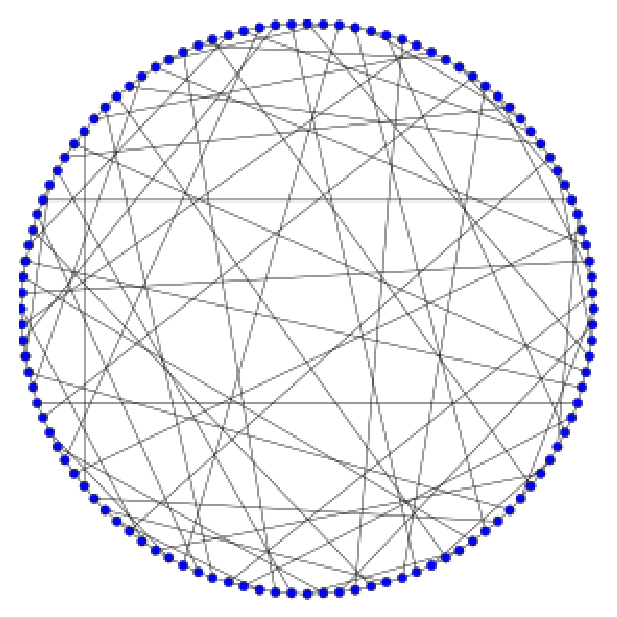
\includegraphics[width=5.7cm]{sample-2b.eps}}
\caption[Title]{\textit{Title.} Caption of this figure. Caption of this figure. Caption of this figure.
Caption of this figure. Caption of this figure. Caption of this figure. Caption of this figure. Caption of this figure.}
\label{fig:subfigures}
\end{figure}
%%

%
% ********************************************
% ********************************************
%

Next paragraph in current heading. Next paragraph in current heading.
Next paragraph in current heading. Next paragraph in current heading.
Next paragraph in current heading. Next paragraph in current heading.
Next paragraph in current heading. Next paragraph in current heading.
Next paragraph in current heading.

% ********************************************
%         Formatting: Tables
% ********************************************
%
% Sample table:
%

%%
\begin{table}[h!]
\captionof{table}[Title]{\textit{Title.} Caption of the table. Caption of the table. Caption of the table.
Caption of the table. Caption of the table. Caption of the table. Caption of the table. Caption of the table. Caption of the table.}
\label{tb:table}
\vspace{-5mm}
\begin{center}
\begin{tabular}{ p{3cm} p{11.4cm} }
\hhline{--}
\rowcolor[gray]{0.9} First line & \\ \hhline{--}
Text & This is the text \\
Text & This is the text \\
Text & This is the text \\
\hhline{--}
\end{tabular}
\end{center}
\end{table}
\vspace{-5mm}
%%

%
% In order to color the first row cell/-s, \rowcolor[gray]{0.9} is used.
% The word 'gray' here denotes the grayscale color scheme, not the color grey and `0.9' denotes how dark the grey is.
%
% The xcolor package provides the necessary commands to produce tables with alternate row colors, when loaded with the table option.
% The command \rowcolors{<starting row>}{<odd color>}{<even color>} has to be specified right before the tabular environment starts.
%
% For footnotes to work inside of tables, apply minipage environment before entering tabular environment.
%
% For more on tables, see
% http://en.wikibooks.org/wiki/LaTeX/Tables
%
% ********************************************
% ********************************************
%

Next paragraph in current heading. Next paragraph in current heading.
Next paragraph in current heading. Next paragraph in current heading.
Next paragraph in current heading. Next paragraph in current heading.
Next paragraph in current heading. Next paragraph in current heading.
Next paragraph in current heading.


Next paragraph in current heading. Next paragraph in current heading.
Next paragraph in current heading. Next paragraph in current heading.
Next paragraph in current heading. Next paragraph in current heading.
Next paragraph in current heading. Next paragraph in current heading.
Next paragraph in current heading.

Next paragraph in current heading. Next paragraph in current heading.
Next paragraph in current heading. Next paragraph in current heading.
Next paragraph in current heading. Next paragraph in current heading.
Next paragraph in current heading. Next paragraph in current heading.
Next paragraph in current heading.

Next paragraph in current heading. Next paragraph in current heading.
Next paragraph in current heading. Next paragraph in current heading.
Next paragraph in current heading. Next paragraph in current heading.
Next paragraph in current heading. Next paragraph in current heading.
Next paragraph in current heading.


Next paragraph in current heading. Next paragraph in current heading.
Next paragraph in current heading. Next paragraph in current heading.
Next paragraph in current heading. Next paragraph in current heading.
Next paragraph in current heading. Next paragraph in current heading.
Next paragraph in current heading.

Next paragraph in current heading. Next paragraph in current heading.
Next paragraph in current heading. Next paragraph in current heading.
Next paragraph in current heading. Next paragraph in current heading.
Next paragraph in current heading. Next paragraph in current heading.
Next paragraph in current heading.

%
% **********************************************
%         Formatting: Algorithms
% **********************************************
%
% In this case, a custom float is used for algorithms (as defined in preamble): myalgorithm
% Any environment can be then used for creation of algorithms when inserted inside the myalgorithm
% environment, e.g. algorithm, algorithmic, algorithm2e, program, verbatim,...
% Sample shows example of program float.

%%
\begin{myalgorithm}[h]
\centering
\caption[Title]{\textit{Title.} Caption of the algorithm. Caption of the algorithm.
Caption of the algorithm. Caption of the algorithm. Caption of the algorithm.
Caption of the algorithm.}
\HRule
\vspace{-9mm}
\begin{program}
\vspace{-2mm}
\mbox{A fast exponentiation procedure:}
\BEGIN %
  \FOR i:=1 \TO 10 \STEP 1 \DO
     |expt|(2,i); \\ |newline|() \OD %
\rcomment{This text will be set flush to the right margin}
\WHERE
\PROC |expt|(x,n) \BODY
          z:=1;
          \DO \IF n=0 \THEN \EXIT \FI;
             \DO \IF |odd|(n) \THEN \EXIT \FI;
\COMMENT{This is a comment statement};
                n:=n/2; x:=x*x \OD;
             \{ n>0 \};
             n:=n-1; z:=z*x \OD;
          |print|(z) \ENDPROC
\END
\end{program}
\vspace{-5mm}
\end{myalgorithm}
\vspace{-2mm}
%%

%
% In case you do not wish to use myalgorithm environment, make sure that the outcome of selected algorithm
% environment used looks as sample below (uncomment between %%). (in this case, also correct the Index of
% Algorithms accordingly).
%
% To see the sample, uncomment between %%

%% \newcommand{\HRule}{\rule{\linewidth}{0.1mm}} % defines line used in the example
%
%\vspace{4mm}
%\noindent{\small{Algorithm 1:                 % set separator as ':'
%\textit{Title of the Algorithm.}              % title of algorithm in italic text
%Caption of the Algorithm.                     % caption of algorithm in plain text on top
%}}
%
%\noindent\HRule
%
%\noindent This is the text.\\
%\noindent This is the text.\vspace{-3mm}\\
%\noindent\HRule
%\vspace{4mm}
%%

% For more on algorithms in algorithm environment, see
% http://en.wikibooks.org/wiki/LaTeX/Algorithms_and_Pseudocode
%
% For more on algorithms in algorithm2e environment, see
% http://www.tug.org/texlive/Contents/live/texmf-dist/doc/latex/algorithm2e/algorithm2e.pdf
%
% ********************************************
% ********************************************
%


Next paragraph in current heading. Next paragraph in current heading.
Next paragraph in current heading. Next paragraph in current heading.
Next paragraph in current heading. Next paragraph in current heading.
Next paragraph in current heading. Next paragraph in current heading.
Next paragraph in current heading.

